% !TEX root = ../dissertation.tex

\chapter{Nonlinear Geometric Control}\label{sec:se3_control}

While there has been significant study of interplanetary transfer trajectories, relatively less analysis has been conducted on operations in the vicinity of asteroids.
The dynamic environment around asteroids is strongly perturbed and challenging for analysis and mission operations~\cite{scheeres1994,scheeres2000}.
Due to their low mass, which results in a low gravitational attraction, asteroids may have irregular shapes and potentially chaotic spin states.
As a result, typical approaches of assuming a inverse square gravitational model are at best inaccurate and at worst do not capture the true dynamic environment.
In addition, the vast majority of asteroid are difficult to track or measure using current ground-based optical sensors. 
Due to their small size, frequently less than \SI{1}{\kilo\meter}, and low albedo the reflected energy of these asteroids is insufficient for reliable detection or tracking.
Therefore, the dynamic model of the asteroid is relatively coarse prior to arrival of a dedicated spacecraft in the vicinity. 
As a result, any spacecraft mission to an asteroid is dependent on a robust dynamic simulation and must incorporate the ability to deal with uncertain forces and environments.

% talk about the coupling between attitude and translational states
Furthermore, since the magnitude of the gravitational attraction is relatively small, non-gravitational effects, such as solar radiation pressure or third-body effects, become much more significant.
As a result, the orbital environment is generally quite complex and it is difficult to generate analytical insights.
One key consideration is the coupling between rotational and translational states around the asteroid.
The coupling is induced due to the different gravitational forces experienced on various parts of the spacecraft.
The effect of the gravitational coupling is related to the parameter \(\epsilon = \frac{r}{R_c}\), where \(r\) is the characteristic spacecraft length and \(R_c\) is the orbital radius~\cite{hughes2004}.
For Earth based missions, the orbital radius is several orders of magnitude larger than the spacecraft length and \(\epsilon\) is small.
As a result, the corresponding gravitational moment is weak and can be neglected. 
Therefore, the translational and rotational equations of motion become decoupled and can be considered separately, significantly simplifying the analysis. 
However, for operations around an asteroid the orbital radius is much smaller, which leads to much larger values of \(\epsilon\) and much larger influence of the rotational and translational coupling.
References~\cite{elmasri2005} and~\cite{sanyal2004} investigated the coupling of an elastic dumbbell spacecraft in orbit about a central body, but only considered the case of a spherically symmetric central body.
Furthermore, the spacecraft model is assumed to remain in a planar orbit.
As result, these developments are not directly applicable to motion about an asteroid, which experience highly non-keplerian dynamics.

% now talk about the specific challenges of asteroid landing. there are lots of trajectory design papers and several have considered landing trajectories
An additional layer of complexity is the design of landing trajectories on asteroids.
Beginning with the first landing of NEAR Shoemaker on asteroid 433 Eros, there has been a concerted effort to develop techniques and methodologies for asteroid landing~\cite{dunham2002, kubota2006}.
There is already considerable knowledge on the planetary landing problem~\cite{acikmese2007, meditch1964, ingoldby1978}.
While conceptually similar, the landing of spacecraft on small bodies requires additional consideration. 
The surface of an asteroid is highly irregular and, as discussed previously, there is a large coupling between the translational and rotational dynamics of the vehicle, which is further exaggerated when close to the surface.
References~\cite{guelman1994, furfaro2013, zexu2012} consider the soft landing problem on an asteroid.
These approaches were primarily based on nonlinear control techniques which allowed for the development of closed loop controllers which enable landing.
However, only the translational dynamics of the body was considered and no notion of the attitude dynamics or it's coupling to the position is considered.
Furthermore, relatively simple gravitational models are used which make the results unsuitable for operations near irregular bodies.
In this chapter, we derive and develop a nonlinear geometric controller for the coupled dynamics of a spacecraft around an asteroid.

An additional layer of complexity is the design of landing trajectories on asteroids.
Beginning with the first landing of NEAR Shoemaker on asteroid 433 Eros, there has been a concerted effort to develop techniques and methodologies for asteroid landing~\cite{dunham2002, kubota2006}.
There is already considerable knowledge on the planetary landing problem~\cite{acikmese2007, meditch1964, ingoldby1978}.
While conceptually similar, the landing of spacecraft on small bodies requires additional consideration. 
The surface of an asteroid is highly irregular and, as discussed previously, there is a large coupling between the translational and rotational dynamics of the vehicle, which is further exaggerated when close to the surface.
References~\cite{guelman1994, furfaro2013, zexu2012} consider the soft landing problem on an asteroid.
These approaches were primarily based on nonlinear control techniques which allowed for the development of closed loop controllers which enable landing.
However, only the translational dynamics of the body was considered and no notion of the attitude dynamics or it's coupling to the position is considered.
Furthermore, relatively simple gravitational models are used which make the results unsuitable for operations near irregular bodies.
\section{Nonlinear Geometric Control}

A wide variety of control schemes have been proposed for asteroid landing missions~\cite{furfaro2013,li2011a}.
In addition, there are a  variety of controllers developed for systems evolving on \( \SE \)~\cite{lee2010,lee2013}.
In this paper, we extend their use from quadrotor aerial vehicles into the space domain. 
This approach addresses many of the issues associated with the related work on asteroid landings.
The geometric control methods used to develop these nonlinear controllers allow for the development of control systems for dynamic systems which evolve on nonlinear manifolds. 
By developing the control system directly on the nonlinear manifold, geometric control techniques provide unique advantages as compared to those developed using local coordinate representations.
Furthermore, the geometric controller avoids the chattering issues inherent in the previous sliding mode control approaches to asteroid landing.
In addition, rather than offering only a bounded stability guarantee, the proposed nonlinear geometric controller guarantees almost global tracking of the attitude and translational states. 
This stability guarantee is critical for mission operations passing close to the surface over highly irregular terrain.
Furthermore, the coupled geometric controller explicitly considers the attitude coupling of the body in contrast to many of the previous approaches.
We briefly summarize the key developments of the \( \SE \) control scheme and leave the detailed derivations to the source manuscripts~\cite{lee2010,lee2013}.
% TODO Basics of geometric control

% TODO Derive attitude and translation control seperately

% TODO Specifics for use in the asteroid case

\subsection{Spacecraft Dynamic Model}\label{sec:controlled_dynamic_model}
We consider the controlled motion of a rigid dumbbell spacecraft about a small body.
% TODO Add some citations for dumbbell for use in spacecraft
The dumbbell spacecraft consists of two masses connected by a massless rod and is a well-known representation of a multi body spacecraft.
Furthermore, the dumbbell model captures the important interactions of the coupling between orbital and attitude dynamics. 
As a result, this simple model is useful to capture the main characteristics of a wide variety of spacecraft configurations.
Typically, spacecraft have mass concentrated in a central structure, referred to as the bus, which houses the command and control system, actuators, fuel, sensors etc. 
In addition, comparatively light-weight solar panels extend from the bus to provide electrical energy from solar radiation. 
As a result, the distributed mass of the spacecraft is captured with the dumbbell representation.
In this section, we briefly review the polyhedron potential model and then present the derivation of the coupled dynamics of a dumbbell spacecraft about an asteroid.
In this work, we assume that the asteroid is much more massive than the spacecraft and its motion is not affected by that of the spacecraft.
This assumption allows us to treat the motion of the vehicle independently from that of the asteroid, instead of treating the more complicated full-body problem. 
% TODO Add link to dynamic model given in previous section
% The spacecraft model is the same as that defined in 

In this section, we develop a coupled control system to track a desired trajectory.
We assume that the desired trajectory, \( R_d(t), \vb{x}_d(t) \), are defined as the rotation matrix of the spacecraft body frame with respect to the inertial frame and the relative position of the spacecraft center of mass with respect to the asteorid and defined in the inertial frame, respectively.
In contrast to controller derived for quadrotor \gls{uav}, the attitude and translational motion is only lightly coupled in the spacecraft scenario.
From the dynamic equations of motion, the coupling between the translational and rotational dynamics is due to the gravitational moment on the spacecraft.
Furthermore, we assume that we have a fully actuated spacecraft such that we can apply a torque about all three rotational axes and a force in all three directions.
This is in contrast to \glspl{uav} where the system is underactuated and in order to produce certain translational forces the system must first rotate.
This is a relatively standard assumption in the astrodynamics community as most spacecraft contain seperate systems for attitude control, e.g.\ \glspl{rwa}, \glspl{cmg}, or cold gas thrusters, and translational control, e.g.\ cold-gas thrusters, electric propulsion, or large chemical rockets~\cite{hughes2004,wertz1978}.
However, there are also many examples of underactuated spacecraft, such as those with damaged components~\cite{petersen2015a} or cubesats with limited cost and/or size budgets.
% TODO Add citaitons for these papers
In these situations, there are a variety of methods to handle the underactuation, ranging from optimal control techniques, exploiting external forces, or utilizing multiple control loops.

The control system is presented as two seperate controllers, one for the attitude tracking and one for translational tracking. 
These controllers are computed independently and used to manuever the spacecraft for both asteroid reconstruction and landing.

\subsection{Attitude Control}
One distinctive feature of the attitude dynamics of rigid bodies is that it evolves on a nonlinear manifold.
The three-dimensional special orthogonal group, or \( \SO \), is the set of \( 3 \times 3 \) orthogonal matrices whose determinant is one.
This configuration space is non-Euclidean and yields unique stability properties which are not observable on a linear space.
For example, it is impossible to achieve global attitude stabilization using continuous time-invariant feedback~\cite{bhat2000}.

Attitude control is typically studied using a variety of attitude parameterizations, such as Euler angles or quaternions~\cite{shuster1993}.
Attitude parameterizations fail to represent the nonlinear configuration space both globally and uniquely~\cite{chaturvedi2011a}.
For example, minimal attitude representations, such as Euler angle sequences or modified Rodriguez parameters, suffer from singularities.
These attitude representations are not suitable for large angular slews.
In order to avoid singularities, the designer must carefully switch the chosen Euler angle sequence based on the operating region.
Another option is to artificially limit the operating region of the rigid body.
This ensures the system operates in a region free from singularities but limits the performance capabilities and ability to perform arbitrarily large angular maneuvers.
Quaternions do not have singularities but they double cover the special orthogonal group.
As a result, any physical attitude is represented by a pair of antipodal quaternions on the three-sphere.
An immediate implication of this ambiguity is that closed-loop stability properties derived using quaternions may not hold for the physical rigid body evolving on the true configuration space, namely the special orthogonal group.
During implementation, the designer must carefully resolve this non-unique representation in quaternion based attitude control systems to avoid undesirable unwinding behavior~\cite{bhat2000}.
This behavior is characterized by situations where the rigid body starts close to the desired attitude, yet the system unnecessarily rotates through a large angle in spite of a small initial error. 

The first step in designing a control system on a nonlinear manifold \( \Q \) is the selection of a proper configuration error function. 
This configuration error function, \( \Psi : \Q \times \Q \to \R \), is a smooth and proper positive definite function that measures the error between the current configuration and a desired configuration. 
Once an appropriate configuration error function is chosen, one can then define a configuration error vector and a velocity error vector in the tangent space \( \mathsf{T}_q \Q \) through the derivatives of \( \Psi \)~\cite{bullo2004}. 
With the configuration error function and vectors, the remaining procedure is analogous to nonlinear control design on Euclidean vector spaces. 
One chooses control inputs as functions of the state through a Lyapunov analysis on \Q.
The configuration error function used in this analysis has been used in~\cite{bullo2004,chaturvedi2009,lee2011a,kulumani2017a}.
In this section we summarize the properties developed previously and present several extensions for our use in the case of motion around an asteroid.

% trackign control
In order to determine the attitude control input, we first define a desired attitude tracking command.
An arbitrary smooth attitude tracking command \( R_d (t) \in \SO \in \R^3 \) are given as a function of time.
% TODO Add link to this equation in dynamic derivation
The corresponding angular velocity command is obtained using the attitude kinematics equation, \( \hat{\Omega}_d = R_d^T \dot{R}_d \).
With the desired attitude command, \( R_d(t), \Omega_d(t) \), we then define the errors associated with the attitude and angular velocity.
The attitude and angular velocity tracking errors must be careful chosen to remain on the tangent bundle of \SO.
\begin{prop}{Attitude Configuration Error Function}\label{prop:attitude_control_configuration_error}
First, an attitude error function \(A : \SO \times \SO  \to \R \), an attitude error vector \( e_R : \SO \times \SO \to \R \), and an angular velocity error \( e_\Omega : \SO \times \R^3 \times \SO \times \R^3 \) are defined as
\begin{subequations}\label{eq:attitude_error_function}
\begin{align}
    A(R, R_d) &= \frac{1}{2} G \tr{I - R_d^T R}, \label{eq:A} \\
    e_R &= \frac{1}{2} G \parenth{R_d^T R - R^T R_d^\vee}, \label{eq:eRA}\\
    e_\Omega &= \Omega - R^T R_d \Omega_d \label{eq:eWA}.
\end{align}
\end{subequations}
Then the following properties hold:
\begin{enumerate}
    \item \label{item:prop_A_psd} \( A \) is locally positive definite about \( R = R_d \) on \( \SO \).
    \item \label{item:prop_eRA} The variation of \( A \) with respect to a variation of \( \delta R = R \hat{\eta} \) for \( \eta \in \R^3 \) is given by
	\begin{align}\label{eq:dirDiff_A}
		\dirDiff{A}{R} &= \eta \cdot e_{R} ,
	\end{align}
	where the notation \( \dirDiff{A}{R} \) represents the directional derivative of $A$ with respect to $R$ along the direction $\delta R$.
    \item \label{item:prop_critical_points} The critical points of \( A \), where \( e_R = 0 \) are \( \braces{R_d} \cup \braces{R_d \exp(\pi \hat s) } \) for \( s \in \braces{e_1, e_2, e_3}\)
    \item \label{item:prop_A_quadratic} \( \Psi \) is a locally quadratic function, which means there exist constants \( 0 < n_1 \leq n_2 \) such that
    \begin{align}\label{eq:A_bound}
        n_1 \norm{e_R}^2 \leq \Psi(R) \leq n_2 \norm{e_R}^2 ,
    \end{align}
    for $0<\psi < h_1 $ where the constants \( n_1 = \frac{h_1}{h_2 + h_3} \) and \( n_2 = \frac{h_1 h_4}{h_5 \parenth{h1 - \psi} }\) for
	\begin{align*}
		h_1 &= \min\braces{g_1 + g_2, g_2 + g_3 , g_3 + g_1} ,\\
		h_2 &= \max\braces{\parenth{g_1 -g_2}^2,\parenth{g_2 -g_3}^2 , \parenth{g_3 -g_1}^2} ,\\
		h_3 &= \max\braces{\parenth{g_1 + g_2}^2, \parenth{g_2 + g_3}^2 , \parenth{g_3 + g_1}^2}, \\		
        h_4 &= \max\braces{g_1 + g_, g_2 +g_3, g+3 + g_1}, \\
        h_5 &= \max\braces{\parenth{g_1 + g_2}^2, \parenth{g_2 + g_3}^2, \parenth{g_3 + g_1}^2}.
	\end{align*}
\end{enumerate}
\end{prop}
\begin{proof}
    See~\Cref{proof:attitude_config_error}
\end{proof}

With the appropriate attitude configuration error we now present the error dynamics in~\cref{prop:attractive_error_dynamics}, which are used in the subsequent development of the nonlinear control system.
\begin{prop}\label{prop:attractive_error_dynamics}
    The attitude error dynamics for \( A(R, R_d), e_\Omega \) satisfy
	\begin{gather}
    	\diff{}{t} \parenth{A(R)} = e_{R_A} \cdot e_\Omega , \label{eq:A_dot} \\
		\diff{}{t} \parenth{e_{R_A}} = E(R, R_d) e_\Omega , \label{eq:eRA_dot} \\
        \diff{}{t} \parenth{e_\Omega} = J^{-1} \parenth{-\Omega \times J \Omega + u + W(R, \Omega) \Delta + M_{ext}} , \label{eq:eW_dot}
	\end{gather}
	where the matrix \(E(R,R_d)\in \R^{3\times3} \) is given by
	\begin{align}
		E(R,R_d) = &\frac{1}{2} \parenth{\tr{R^T R_d G}I - R^T R_d G} , \label{eq:E} \\
	\end{align}
\end{prop}
\begin{proof}
    See~\Cref{proof:attractive_error_dynamics}
\end{proof}

\subsubsection{Attitude Control without Disturbance}
With the appropriate attitude configuration error we now present an attitude controller for attitude stabailization and tracking. 
This controller assumes that there is no disturbances on the attitude dynamics, i.e.\ \( \Delta = 0 \).
\begin{prop}[Attitude Control]\label{prop:att_control}
	Given a desired attitude command \( \parenth{R_d, \Omega_d = 0} \) and positive constants \( k_R, k_\Omega \in \R \) we define a control input \( u \in \R^3 \) as follows
	\begin{gather}
        u = -k_R e_R - k_\Omega e_\Omega + \Omega \times J \Omega - M_{ext}. \label{eqn:nodist_control}
	\end{gather}
	Then the zero equilibrium of the attitude error is asymptotically stable, and the inequality constraint is always satisfied.
\end{prop}
\begin{proof}
See~\Cref{proof:att_control}
\end{proof}

\subsection{Constrained Attitude Control}

Many physical rigid body systems must perform large angular slews in the presence of state constraints.
For example, autonomous spacecraft or aerial systems are typically equipped with sensitive optical payloads, such as infrared or interferometric sensors.
These systems require retargeting while avoiding direct exposure to sunlight or other bright objects.
In addition, many ground based attitude testing environments, such as air bearing platforms, must operate in the presence of physical obstructions.
Determining a satisfactory attitude control maneuver in the presence of state constraints is a challenging task.
The removal of constrained regions from the rotational configuration space results in a \textit{nonconvex} region.
The attitude control problem in the feasible configuration space has been extensively studied~\cite{bullo2004,MayTeePaCC11,LEEITAC15}.
However, the attitude control problem in the presence of constraints has received much less attention.

% discuss how previous papers (mcinnes and lee/meshabi) have short comings
Several approaches have been developed to treat the attitude control problem in the presence of constraints.
A conceptually straightforward approach is used in~\cite{hablani1999} to determine feasible attitude trajectories prior to implementation.
The algorithm determines an intermediate point such that an unconstrained maneuver can be calculated for each subsegment.
Typically, an optimal or easily implementable on-board control scheme for attitude maneuvers is applied to maneuver the vehicle along these segments.
In this manner, it is possible to solve the constrained attitude control problem by linking several intermediary unconstrained maneuvers.
While this method is conceptually simple, it is difficult to generalize for an arbitrary number of constraints.
In addition, this approach is only applicable to problems where the selection of intermediate points are computationally feasible.

The approach in~\cite{frazzoli2001} involves the use of randomized motion planning algorithms to solve the constrained attitude control problem.
A graph is generated consisting of vertices from an initial attitude to a desired attitude. 
A random iterative search is conducted to determine a path through a directed graph such that a given cost, which parameterizes the path cost, is minimized.
The random search approach can only stochastically guarantee attitude convergence as it can be shown that as the number of vertices in the graph grow, the probability of nonconvergence goes to zero.
However, the computational demand grows as the size of the graph is increased and a new graph is required when constraints are modified. 
As a result, random search approaches are ill-suited to on-board implementation or in scenarios that require agile maneuvers.

Model predictive control for spacecraft attitude dynamics is another popular approach and has been studied in~\cite{guiggiani2014,kalabic2014,gupta2015}.
These methods rely on linear or non-linear state dynamics to repeatedly solve a finite-time optimal control problem.
Also known as receding horizon control, the optimal control formulation allows for a straight forward method to incorporate state and control constraints.
Computing the optimal control strategy over a moving horizon allows for a form of feedback type control rather than the more typical open-loop optimal control solution.
Due to the iterative nature of solving optimization problems, model predictive control methods are computational expensive and frequently apply direct optimization methods to solve the necessary conditions for optimality.
Therefore, these methods are complicated to implement and may not be suitable for real-time control applications.
  
% Previous potential function approach - developed using attitude parameterizations - singularities/ambiguities
Artificial potential functions are commonly used to handle kinematic constraints for a wide range of problems in robotics~\cite{rimon1992}.
The goal is the design of attractive and repulsive terms which drive the system toward or away from a certain obstacle, respectively.
The attractive function is designed to drive the system towards the desired state.
Similarly, a repulsive function is constructed such that the system is directed away from the constraints. 
The superposition of these functions allows one to apply standard feedback control schemes for stabilization and tracking.
More specifically, artificial potential functions have previously been applied to the spacecraft attitude control problem in~\cite{lee2011b,mcinnes1994}.
However, both of these approaches were developed using attitude parameterizations, namely Euler angles and quaternions, and as such, they are limited by the singularities of minimal representations or the ambiguity of quaternions.

This section is focused on developing an adaptive attitude control scheme in the presence of attitude inequality constraints on \(\SO\).
We apply a potential function based approach developed directly on the nonlinear manifold \(\SO\). 
By characterizing the attitude both globally and uniquely on \(\SO\), our approach avoids the issues of attitude parameterizations, such as kinematic singularities and ambiguities, and is geometrically exact. 
A configuration error function on \(\SO\) with a logarithmic barrier function is proposed to avoid constrained regions. 
Instead of calculating a priori trajectories, as in the randomized approaches, our approach results in a closed-loop attitude control system. 
This makes it ideal for on-board implementation on UAV or spacecraft systems. 
In addition, unlike previous approaches our control system can handle an arbitrary number of constrained regions without modification.
This approach results in a conceptually simple obstacle avoidance scheme which extends the previous work of artificial potential functions on Euclidean spaces to the special orthogonal group.
Furthermore, we use this new configuration error function to design an adaptive update law to enable attitude convergence in the presence of uncertain disturbances. 

\paragraph{State Inequality Constraint}\label{sec:state_inequality_constraint}
The two-sphere is the manifold of unit-vectors in \( \R^3 \), i.e., \( \Sph^2 = \{ q \in \R^3 \,  \vert \, \norm{q} = 1 \}\).
We define \( r \in \Sph^2 \) to be a unit vector from the mass center of the rigid body along a certain direction and it is represented with respect to the body-fixed frame.
For example, \( r \) may represent the pointing direction of an on-board optical sensor.
We define \( v \in \Sph^2 \) to be a unit vector from the mass center of the rigid body toward an undesired pointing direction and represented in the inertial reference frame.
For example, \( v \) may represent the inertial direction of a bright celestial object or the incoming direction of particles or other debris.
It is further assumed that optical sensor has a strict non-exposure constraint with respect to the celestial object.
We formulate this hard constraint as
\begin{align}
	r^T R^T v \leq \cos \theta , \label{eqn:constraint}
\end{align}
where we assume \( \ang{0} \leq \theta \leq \ang{90}  \) is the required minimum angular separation between \( r \) and \( R^T v \). 
The objective is to a determine a control input \( u \) that stabilizes the system from an initial attitude \( R_0 \) to a desired attitude \( R_d \) while ensuring that~\cref{eqn:constraint} is always satisfied.

\paragraph{Constrained Attitude Error Function}
To handle the attitude inequality constraint, we propose a new attitude configuration error function. 
More explicitly, we extend the trace form used in~\cite{bullo2004,LeeITCST13} and presented in~\Cref{prop:attitude_control_configuration_error} for attitude control on \(\SO\) with the addition of a logarithmic barrier function. 
Based on the proposed configuration error function, a nonlinear geometric attitude controller is constructed. 
A smooth control system is first developed assuming that there is  no disturbance, and then it is extended to include an adaptive update law for stabilization in the presence of unknown disturbances. 
The proposed attitude configuration error function and several properties are summarized as follows.
\begin{prop}[Constrained Attitude Error Function] \label{prop:repulsive_configuration_error}
Define an attitude error function \( \Psi : \SO \to \R \), an attitude error vector \( e_R \in \R^3 \), and an angular velocity error vector \( e_\Omega \in \R^3 \) as follows:
\begin{gather}
	\Psi(R, R_d) = A(R, R_d) B(R) , \label{eq:psi} \\
	e_R = e_{R_A} B(R) + A(R,R_d) e_{R_B} , \label{eq:eR} \\
	e_\Omega = \Omega , \label{eq:eW}
\end{gather}
with
\begin{gather}
	B(R) = 1 - \frac{1}{\alpha} \ln \left( \frac{\cos \theta -  r^T R^T v}{1 + \cos \theta}\right). \label{eq:B} \\
	e_{R_B} = \frac{\left( R^T v\right)^\wedge r}{\alpha \left(r^T R^T v - \cos \theta \right)}. \label{eq:eRB} 
\end{gather}	
where \( \alpha \in \R \) is defined as a positive constant.
Then, the following properties hold
\begin{enumerate}
	\item \label{item:prop_psi_psd} \(\Psi\) is positive definite about \( R = R_d\) on $\SO$.
	\item \label{item:prop_erb} The variation of \( B(R) \) with respect to a variation of \( \delta R = R \hat{\eta} \) for \( \eta \in \R^3 \) is given by
	\begin{align}\label{eq:dirDiff_B}
		\dirDiff{B}{R} &= \eta \cdot e_{R_{B}}.
	\end{align}
    \item \label{item:prop_psi_quadratic} \( \Psi \) is a locally quadratic function, which means there exist constants \( 0 < n_1 \leq n_2 \) such that
    \begin{align}\label{eq:psi_bound}
        n_1 \norm{e_R}^2 \leq \Psi(R) \leq n_2 \norm{e_R}^2 ,
    \end{align}
    on the neighborhood $D$ of the desired attitude \( R_d \)
    \begin{align}\label{eq:psi_quadratic_domain}
        D = \braces{R\in\SO  \vert \Psi < \psi < h_1, r^T R^T v < \beta < \cos \theta}
    \end{align}
    for $0<\psi < h_1 $ and $0< \beta<\cos\theta$. 
\end{enumerate}
\end{prop}
\begin{proof}
    See~\Cref{proof:repulsive_configuration_error}
\end{proof}

\Cref{eqn:psi} is composed of an attractive term, \( A (R) \) toward the desired attitude, and a repulsive term, \( B(R) \) away from the undesired direction \( R^T v \).
In order to visualize the attitude error function on \( \SO \), we utilize a spherical coordinate representation.
Recall, that the spherical coordinate system represents the position of a point relative to an origin in terms of a radial distance, azimuth, and elevation.
This coordinate system is commonly used to define locations on the Earth in terms of a latitude and longitude.
Similarly, the positions of celestial objects are defined on the celestial sphere in terms of right ascension and declination. 
\begin{figure}[htbp]%
    \centering 
    \subcaptionbox{Attractive \( A(R) \) \label{fig:attract_error} }{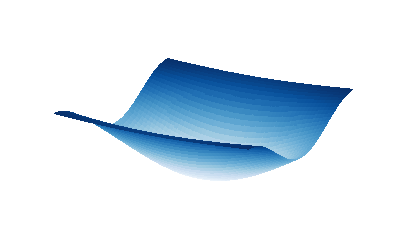
\includegraphics[trim={8mm 2mm 8mm 2mm}, clip, width=0.3\textwidth]{figures/2016_IJCAS/attract_error.pdf}}
    \subcaptionbox{Repulsive \( B(R) \) \label{fig:avoid_error} }{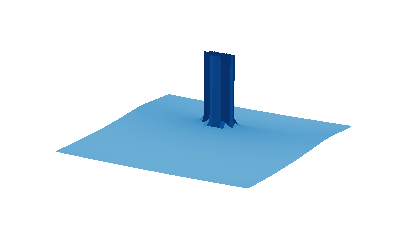
\includegraphics[trim={8mm 2mm 8mm 2mm}, clip, width=0.3\textwidth]{figures/2016_IJCAS/avoid_error.pdf}}
    \subcaptionbox{Combined \( \Psi \) \label{fig:combined_error} }{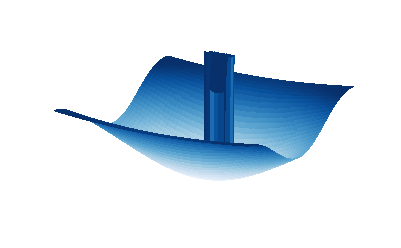
\includegraphics[trim={8mm 2mm 8mm 2mm}, clip, width=0.3\textwidth]{figures/2016_IJCAS/combined_error.pdf}}%
    \caption{Visualization of Configuration Error Functions using spherical coordinate representation}
    \label{fig:config_error} 
\end{figure}%
We apply this concept and parameterize the rotation matrix \( R \in \SO \) in terms of the spherical angles \( \SI{-180}{\degree} \leq \lambda \leq \SI{180}{\degree}  \) and \( \SI{-90}{\degree} \leq \beta \leq \SI{90}{\degree} \). 
Using the elementary Euler rotations, the rotation matrix is now defined as \( R = \exp( \lambda \hat{e}_2) \exp( \beta \hat{e}_3) \).
We iterate over the domains of \( \lambda\) and \(\beta\) in order to rotate the body-fixed vector \( r \) throughout the two-sphere \( \S^2 \).
Applying this method,~\cref{fig:config_error} allows us to visualize the error function on \( \SO \).
The horizontal axes of~\cref{fig:config_error} represent the domain of the spherical angles \( \lambda \) and \( \beta \) in degrees, while the vertical axes represent the unitless magnitude of the error functions defined in~\cref{eq:psi,eq:A,eq:B}.
The attractive error function, given by~\cref{eq:A}, has been previously used for attitude control on \(\SO\).
The potential well of \( A(R)\) is illustrated in~\cref{fig:attract_error}, where the desired attitude lies at the minimum of \( A(R) \).

To incorporate the state inequality constraints we apply a logarithmic barrier term.
Barrier functions are typically used in optimal control and motion planning applications.
A visualization of the repulsive error function is presented in~\cref{fig:avoid_error} which shows that as the boundary of the constraint is neared, or \( r^T R^T v \to \cos \theta \), the barrier term increases, \( B \to \infty\).
We use the scale factor~\(\frac{1}{1+\cos \theta} \) to ensure that \( \Psi \) remains positive definite.
The logarithmic function is popular as it quickly decays away from the constraint boundary.
The positive constant \( \alpha \) serves to shape the barrier function.
As \( \alpha \) is increased the impact of \( B(R) \) is reduced away from the constraint boundary. 
The superposition of the attractive and repulsive functions is shown in~\cref{fig:combined_error}.
The control system is defined such that the attitude trajectory follows the negative gradient of \( \Psi \) toward the minimum at \( R = R_d \), while avoiding the constrained region.

While~\cref{eqn:B} represents a single inequality constraint given as~\cref{eqn:constraint}, it is readily generalized to multiple constraints of an arbitrary orientation. 
For example, the configuration error function can be formulated as $\Psi=A[1+\sum_i C_i]$, where $C_i$ has the form of $C_i=B-1$ for the $i$-th constraint. 
In this manner, one may enforce multiple state inequality constraints, and we later demonstrate this through numerical simulation. 
This is in contrast to many previous approaches which are computationally difficult to extend to situations with multiple constraints.
We present the dynamics of the combined configuration error function in~\Cref{prop:error_dyn}, which are used in the subsequent development of the nonlinear control system.

\begin{prop}[Constrained Error Dynamics]\label{prop:repulsive_error_dynamics}
	The attitude error dynamics for \( \Psi, e_R, e_\Omega \) satisfy 
	\begin{gather}
		\diff{}{t} \parenth{\Psi} = e_R \cdot e_\Omega , \label{eq:psi_dot}\\
		\diff{}{t} \parenth{e_R} = \dot{e}_{R_A} B + e_{R_A} \dot{B} + \dot{A}e_{R_B} + A \dot{e}_{R_B} , \label{eq:eR_dot} \\
		\diff{}{t} \parenth{e_{R_B}} = F(R) e_\Omega , \label{eq:eRB_dot} \\
		\diff{}{t} \parenth{B(R)} = e_{R_B} \cdot e_\Omega , \label{eq:B_dot} \\
	\end{gather}
	where the matrix \(F(R) \in \R^{3\times3} \) is given by
	\begin{align}
		F(R) = &\frac{1}{\alpha \parenth{r^T R^T v - \cos \theta}} \left[\parenth{v^T R r} I - R^T v r^T + \frac{R^T \hat{v} R r v^T R \hat{r}}{\parenth{r^T R^T v - \cos \theta}}\right]. \label{eq:F}
	\end{align}
\end{prop}
\begin{proof}
    See~\Cref{proof:repulsive_configuration_error}.
\end{proof}

We extend the results of the controller presented in~\cref{prop:att_control} with the addition of a fixed but unknown disturbance \( \Delta \).
This scenario is typical of many mechanical systems and represents unmodelled dynamics or external moments acting on the system.
For example, Earth orbiting spacecraft typically experience a torque due to a gravitational gradient.
% as well as external torques to due solar radiation pressure.
Aerial vehicles will similarly experience external torques due to air currents or turbulence.
An adaptive control system is introduced to asymptotically stabilize the system to a desired attitude while ensuring that state constraints are satisfied. %We first show several properties of the controlled system. 
\begin{prop}[Bound on \( \bm{\dot{e}_R} \)]\label{prop:eR_dot_bound}
Consider the neighborhood \( D \), given in~\cref{prop:repulsive_configuration_error}, about the desired attitude, then the following statements hold:
\begin{enumerate}
    \item \label{item:prop_eR_dot_bound_AB} Upper bounds of \( A(R) \) and \( B(R) \) are given by
        \begin{gather}
            \norm{A} < b_2 \norm{e_{R_A}}^2 < c_A  , \quad \norm{B} < c_B. \label{eqn:AB_bound}
        \end{gather}
        where the constant \( b_2\) is given by \( b_2 = \frac{h_1 h_4}{h_5 \parenth{h_1 - \psi}}\) for
        \begin{align*}
            h_4 &= \min\braces{g_1 + g_2, g_2 + g_3 , g_3 + g_1} ,\\
            h_5 &= \min\braces{\parenth{g_1 + g_2}^2,\parenth{g_2 + g_3}^2 , \parenth{g_3 + g_1}^2}.\\
        \end{align*}
    \item \label{item:prop_eR_dot_bound_EF} Upper bounds of \( E(R,R_d) \) and \( F(R) \) are given by
        \begin{gather}
            \norm{E} \leq \frac{1}{\sqrt{2}} \tr{G}  , \label{eqn:E_bound} \\
            \norm{F} \leq \frac{\parenth{\beta^2 + 1}\parenth{\beta - \cos \theta}^2 + 1 + \beta^2 \parenth{\beta^2-2}}{\alpha^2 \parenth{\beta-\cos \theta}^4}. \label{eqn:F_bound}
        \end{gather}
    \item Upper bounds of the attitude error vectors \( e_{R_A} \) and \( e_{R_B} \) are given by
        \begin{gather}
            \norm{e_{R_A}} \leq \sqrt{\frac{\psi}{b_1}}, \label{eqn:eRA_bound} \\
            \norm{e_{R_B}} \leq \frac{\sin\theta}{\alpha \parenth{\cos \theta - \beta}}. \label{eqn:eRB_bound}
        \end{gather}
\end{enumerate}
These results are combined to yield a maximum upper bound of the time derivative of the attitude error vector \( \dot{e}_R \) as
\begin{gather}
	\norm{\dot{e}_R} \leq H \norm{e_\Omega} ,\label{eqn:eR_bound}
\end{gather}
where  \( H \in \R \) is defined as
\begin{gather}
	H = \norm{B} \norm{E} + 2 \norm{e_{R_A}} \norm{e_{R_B}} + \norm{A}\norm{F}. \label{eqn:H}
\end{gather}
\end{prop}
\begin{proof}
See~\Cref{proof:eR_dot_bound}
\end{proof}

Adaptive control is typically used in dynamical systems with varying or uncertain components.
In~\Cref{prop:adaptive_control}, we present an adaptive attitude controller which handles uncertain disturbances while satisfying the state inequality constraints.
\begin{prop}[Constrained Adaptive Attitude Control]\label{prop:adaptive_control}
Given  a desired attitude command \( (R_d, \Omega_d = 0 )\) and positive constants \( k_R, k_\Omega, k_\Delta, c \in \R \), we define a control input \( u \in \R^3\) and an adaptive update law for the estimated uncertainty \( \bar{\Delta} \) as follows:
\begin{align}
    u &= - k_R e_R - k_\Omega e_\Omega + \Omega \times J \Omega - W \bar{\Delta} - M_{ext} , \label{eqn:adaptive_control} \\
	\dot{\bar{\Delta}} &= k_\Delta W^T \parenth{e_\Omega + c e_R} . \label{eqn:delta_dot}
\end{align}
If \( c \) is chosen such that
\begin{gather}
	0 < c < \min \braces{\sqrt{\frac{2 \lambda_m k_R n_1}{\lambda_M^2}},
	%\sqrt{\frac{2 k_R n_2}{\lambda_M}}, 
	\frac{4 k_R k_\Omega}{k_\Omega^2 + 4 k_R \lambda_M H}} , \label{eqn:c_bound}
\end{gather}
  the zero equilibrium of the error vectors is stable in the sense of Lyapunov. Furthermore, $e_R,e_\Omega\rightarrow 0$ as $t\rightarrow\infty$, and $\bar\Delta$ is  bounded.
\end{prop}
\begin{proof}
See~\Cref{proof:adaptive_control}
\end{proof}


\subsection{Attitude Pointing modes}

This positive definite function parameterizes the error between the current attitude, \( R \), and the desired attitude command \( R_d \).
Using the variations of \( \Psi \) gives the attitude tracking error vector \( e_R \in \R^3 \) as
\begin{align}\label{eq:attitude_error_vector}
    e_R = \frac{1}{2} \parenth{R_d^T R - R^T R_d^\vee}.
\end{align}
After further manipulation and using the attitude kinematics equation from~\cref{eq:attitude_kinematics}, it is possible to define the angular veloicty tracking error \( e_\Omega \in \R^3 \) as
\begin{align}\label{eq:angular_velocity_error_vector}
    e_\Omega = \Omega - R^T R_d \Omega_d.
\end{align}
With the properly defined attitude error vectors the rotational control input is defined as 
\begin{align*}\label{eq:rotational_control}
    \vb{u}_m = - k_R e_R - k_\Omega e_\Omega + \Omega \times J \Omega - J \parenth{\hat{\Omega} R^T R_d \Omega_d - R^T R_d \dot{\Omega}_d} - \vb{M}_1 - \vb{M_2} 
\end{align*}
where \( k_R, k_\Omega \) are positive controller constants.

\subsection{Translation Control}
The translational control input is defined in a similar manner. 
First we define a smooth tracking command \( x_d(t) \in \R^3 \), which defines the desired position of the spacecraft in the inertial frame.
The tracking error vectors are easier to define as they evolve on a Euclidean space rather than a nonlinear manifold and are given by
\begin{align}
    e_x = x - x_d ,\\
    e_v = v - \dot{x}_d.
\end{align}
With the error variables, the translational control input is then given by
\begin{align}\label{eq:translation_control}
    \vb{u}_f = - k_x e_x  - k_v e_v + ( m_1  + m_2 ) \ddot{x}_d - \vb{F}_1 - \vb{F}_2 ,
\end{align}
where \( k_x, k_v \) are positive constants. 
The control gains are chosen based on the desired closed-loop system response. 
A variety of techniques are available to choose these gains, but a simple linear analysis offers a straightforward and systematic approach to choosing suitable values. 
We use the control inputs defined in~\cref{eq:translation_control,eq:rotational_control} and substitute them into the dynamic equations of motion in~\cref{eq:translational_dynamics,eq:attitude_dynamics}.
This results in the dynamics of the error variables and the gains are chosen to ensure the error behavior meets desired performance criteria, such as percent overshoot or settling time~\cite{nise2004}.


\section{Numerical Example}

% TODO Disucss numerical implementation
Typically, spacecraft missions require extensive interaction from ground based human operators. 
This interaction ranges from system health checks to navigation and hardware commands.
In addition, there is frequently a large group of analysts in support of any given mission. 
A wide variety of factors make human in the loop control of spacecraft especially difficult.
First, the vast distances cause significant time delays which render it impossible to react immediately to events experienced by the spacecraft. 
Furthermore, deep space missions are designed for continuous mission operations for many years or even decades. 
It is becoming increasingly difficult to maintain trained and knowledgeable staff for several decades in order to support a single mission.
In addition, these operators become increasingly scarce as the contemporary hardware and software tools surpass those of these decades old spacecraft. 
As a result, there is a large focus on completely autonomous spacecraft systems.

We present a numerical simulation of a rigid dumbbell about asteroid Itokawa.
The dumbbell spacecraft is composed of two equal masses, \( m_1, m_2 = \SI{500}{\kilo\gram} \), seperated by \( l = \SI{3}{\meter} \).
The dumbbell body frame is defined with the first body fixed axis, \( \vb{b}_1 \), originating at the center of mass of the spacecraft and directed along the vector from \( m_1 \) towards \( m_2 \).
The other two axes of the spacecraft fixed frame are chosen orthogonal to the \( \vb{b}_1 \) and lie in the plane orthogonal to the dumbbell axis of symmetry. 
A camera, using the parameters from~\cref{tab:camera_parameters}, is aligned with the \( \vb{b}_1 \) axis and used to feed image data to the ORB-SLAM system.
A numerical simulation is used to demonstrate the geometric control of the coupled motion of the spacecraft, and the ability to estimate the motion of the spacecraft from monocular imagery.

The initial condition of the spacecraft is defined as
\begin{align}
    \vb{x}_0 &= \begin{bmatrix} 0 & -2.550 & 0 \end{bmatrix} \si{\kilo\meter}, \\
    R_0 &= \exp {\frac{\pi}{2} \vb{e}_3}.
\end{align}
The spacecraft begins on the inertial \( \vb{e}_2 \) axis and initially pointing at the asteroid. 
A tracking command is designed to transition the spacecraft towards the asteroid fixed \( \vb{f}_1  \) axis followed by a vertical descent along towards the asteroid surface.
The translational command is divided into two stages, a traverse step where the spacecraft follows a trajectory to align itself with the \( \vb{f}_1 \) axis and a landing step where the spacecraft follows a constant velocity descent towards the surface. 
The desired position command is defined as
\begin{align}
    \vb{x}_d = 
    \begin{cases}
        2.550 \begin{bmatrix} \sin{\omega t} & -\cos{\omega t} & 0 \end{bmatrix}, & t \leq t_d \\
        R_A \begin{bmatrix} \frac{2}{t_d} (t - t_d) + 2.550 & 0 & 0 \end{bmatrix}, & t > t_d , 
    \end{cases}
\end{align}
where \( \omega = \frac{\pi}{2 t_d} \), \( t_d \) is the time from the simulation start when the constant velocity descent should begin, and \( t \) is the simulation time step.

The desired attitude command is chosen such that the spacecraft camera axis, \( \vb{b}_1 \), is directed along the nadir towards the asteroid.
It is sufficient to define two orthogonal vectors to uniquely determine the attitude of the spacecraft.
The \( \vb{b}_{3d} \) vector is chosen to lie in the plane spanned by \(\vb{b}_{1d} \) and \( \vb{e}_3 = \vb{f}_3 \).
The desired attitude command is defined as
\begin{align}
    \vb{b}_{1d} &= - \frac{\vb{x}}{\norm{\vb{x}}} , \\
    \vb{b}_{3d} &= \frac{\vb{f}_3 - \parenth{\vb{f}_3 \cdot \vb{b}_{1d}} \vb{b}_{1d}}{\norm{\vb{f}_3 - \parenth{\vb{f}_3 \cdot \vb{b}_{1d}} \vb{b}_{1d}}}, \\
    \vb{b}_{2d} &= \vb{b}_{3d} \times \vb{b}_{1d} , \\
R_d &= \begin{bmatrix} \vb{b}_{1d} & \vb{b}_{2d} & \vb{b}_{3d} \end{bmatrix}.
\end{align}
The camera axis is aligned with the spacecraft \( \vb{b}_ 1 \) axis, which is direted towards the asteroid, throughout the landing trajectory as the spacecraft moves in the equatorial plane of the asteroid.

The simulation is carried out over \SI{7200}{\second} with the spacecraft following a circular trajectory for the first \SI{3600}{\sec} before vertically descending in the body fixed frame for the last \SI{3600}{\second}.
\Cref{fig:true_landing_trajectory} shows a view from the positive \( \vb{f}_3 \) pole of the asteroid of the simulated trajectory. 
The position of the center of mass of the dumbbell is shown in blue, while the pointing direction of the camera axis is defined in red. 
The attitude of the dumbbell is displayed at several points along the trajectory demonstraiting the pointing of the camera. 
Furthermore, asteroid Itokawa is shown in its final orientation at the completion of the landing simulation. 
\Cref{fig:pos_components} shows that the nonlinear controller is able to accurately track the desired translational trajectory for the duration of the simulation.
\begin{figure}[htbp]
    \captionsetup[subfigure]{position=b}
    \centering
    \subcaptionbox{Planar view of landing trajectory\label{fig:true_landing_trajectory}}{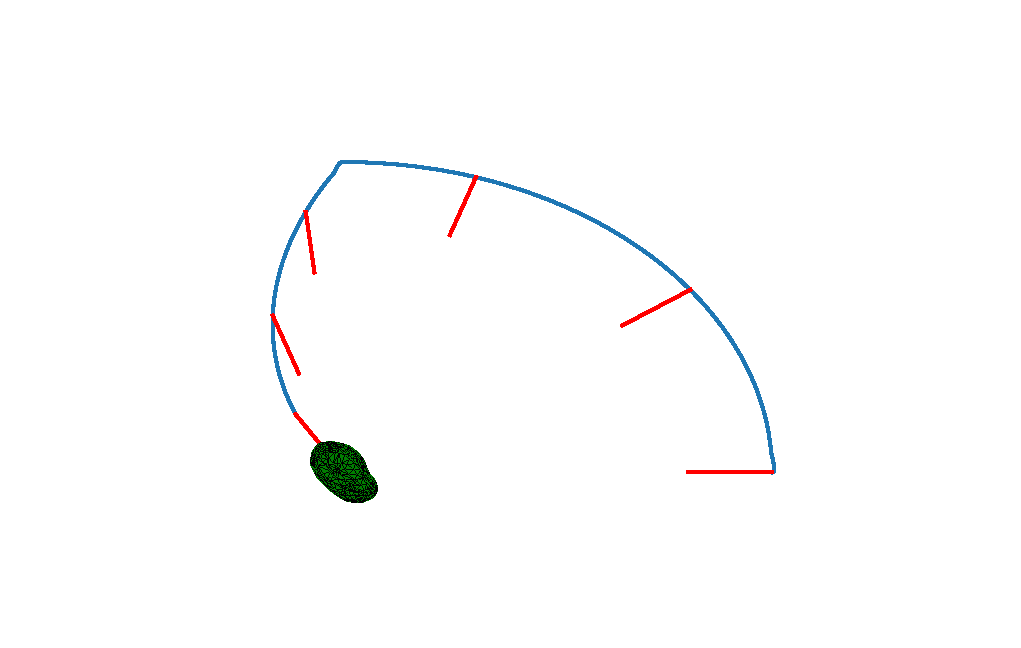
\includegraphics[width=0.5\textwidth]{figures/2017_AAS_fall/traj_fig.pdf}}
    \subcaptionbox{Position of spacecraft in the inertial frame\label{fig:pos_components}}{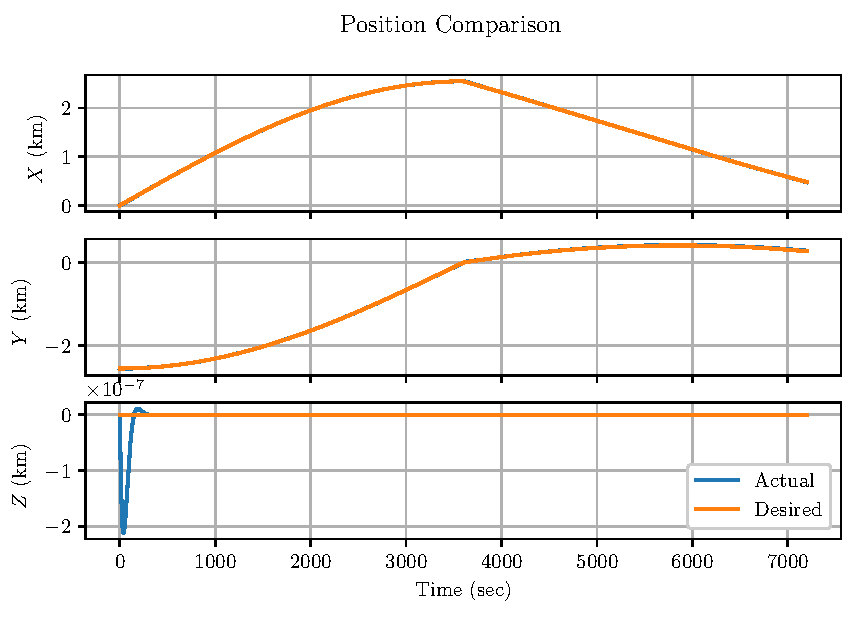
\includegraphics[width=0.5\textwidth]{figures/2017_AAS_fall/pos_fig.pdf}}
    \caption{Landing trajectory to asteroid Itokawa~\label{fig:position}}
\end{figure}
